\subsubsection{Man in the Middle (MITM)}
The man in the middle attack puts the attacker between the station and the access point, allowing them to eavesdrop on communications taking place. In wireless communications, monitoring passing traffic is trivial considering traffic is broadcast and picked up by all network cards in the vicinity; but usually discarded if not intended recipient. This attack allows the attacker easy access to user data sent over unencrypted protocols such as HTTP, but also allows them to use tools such as sslstrip [1] to attempt to thwart HTTPS.

\begin{figure}[h!]
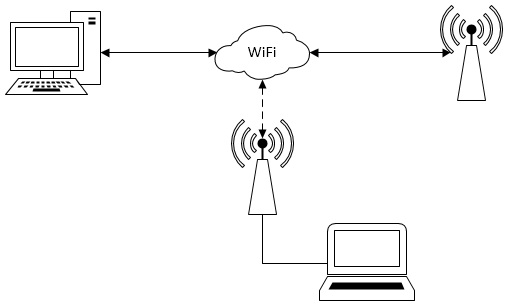
\includegraphics[width=\linewidth]{research/figures/mitm.png}
\caption{Malicious user monitors and injects data packets in to traffic.}
\end{figure}

This style of attack is a popular choice when communications involve some type of public key encryption. 

A more recent variation to this attack, that reflects the shift toward web applications, is the Man in the Browser (MitB). The advantage this has over the vanilla MITM attack is SSL style authentication measures do not hinder its effectiveness. Examples of the MitB attack include HTTP Cache Poisoning [3] and HTTP Response Splitting [4], both can leave lasting effects on the browser in question.

This attack will feature in the project implementation as a means of inspecting leaked data from applications when stations are caught in the honeypot.
